\documentclass{beamer}
\usepackage{pgfpages}
\usepackage{url}
\usepackage[round]{natbib}

\setbeameroption{show notes on second screen}
\setbeamertemplate{caption}[numbered]

\urldef{\incidentDashboard}\url{https://julianbarg.shinyapps.io/incident_dashboard/}

\title{Valuing Peace and Quiet: the Effect of Expansion Mode on Learning toward Subordinate Goals}
\author{Julian Barg}
\institute{Ivey Business School}
\date{Sept 27, 2019}
\logo{
\includegraphics[scale=0.08]{resources/ivey_logo.jpg}}

\begin{document}
	
\frame{\titlepage}

\begin{frame}
	\frametitle{Outline}
	\tableofcontents
\end{frame}

\begin{frame}
	\frametitle{Summary}
	\begin{block}{Findings}
		\begin{itemize}
			\item Organization-wide strategic changes will disrupt learning that has occurred in suborganizations.
			\note{This is what expansion mode refers to in the title, not greenfield or M\&A (although there are M\&As in the dataset).\\\medskip}
			\item Thus, when "nothing happens", something does happen: organizational learning.
			\item From a learning perspective, it is better to take a long-term perspective on strategic adjustments.
				\begin{itemize}
					\item Implementing change in a less disruptive fashion.
				\end{itemize}
				\note{"Learning perspective" matters, because from a technology perspective, the conclusion might be different.}
			\item Depending on the context, implications for organizational performance (environmental and economic).
			\note{In a temporality-inspired learning research fashion. Depending on the type of organization - where mistakes threaten survival, very relevant.}
		\end{itemize}
	\end{block}
\end{frame}

\section{Context}

\begin{frame}
	\frametitle{Context}
	\pipelinesDashboard
	\note{"This is a tool I use for my research." Just briefly show the nature of the data.
		\begin{itemize}
			\item We have comprehensive data on pipelines in the US.
			\item We know which organizations have how many miles. (show top 5)
			\item We know how old their pipelines are.
			\item We know how many incidents occur.
			\item So it would be a great context to study strategy, and how it affects incident rates.
		\end{itemize}}
\end{frame}

\begin{frame}
	\frametitle{Cases}
	\incidentDashboard
	\note{"This is a tool I use for my research." Just briefly show the scale, because i found it hard to imagine, just from numbers.
		\begin{itemize}
			\item Show all organizations at once, add some jitter, alpha.
			\item Show one group, remove jitter, alpha.
		\end{itemize}}
\end{frame}

\begin{frame}
	\frametitle{Context}
	\begin{block}{High-profile bankruptcies related to pipeline incidents}
		\begin{itemize}
			\item Greka Energy/HVI Cat Canyon (1996, 2005, 2019)
			\note{Greka: History of oil spills, settlements relatively unexpensive, e.g., \$12 million fine caused bankruptcy in 2019, ironically, CEO once stated company motto as "Working for profits".\medbreak}
			\item Pacific Gas and Electric Company (2001, 2019)
			\note{PG\&E: After 2010 explosion with 8 deaths, paid \$300m in fines, \$400m in refunds, \$850m for upgrades, and \$500m in settlements.\medbreak}
			\item{EdgeMark (2019)}
			\note{EdgeMark: Energy Transfer pipeline explosion led to EdgeMark Bankruptcy. Ontario Teachers' Pension fund held minority stake. \bigbreak}
		\end{itemize}	
	\end{block}

	\hrulefill
	
	$\rightarrow$ There is some relevance for traditional performance also.
	\note{\hrulefill \smallbreak
		I don't explore this relevance for performance any further though.}
\end{frame}


\section{Learning}

\begin{frame}
	\frametitle{Organizational forgetting: Definitions}
	\begin{itemize}
		\item \textit{Organizational learning}: "change in the organization's knowledge that occurs as a function of experience" \citep[p. 31]{Argote2013}.
		\item \textit{Organizational forgetting}: "the loss, voluntary or otherwise, of organizational knowledge [which] often leads to a change in organizational capabilities because of the absence of some piece of knowledge" \citep[p. 1606]{DeHolan2004}.
		\note{Both forgetting and disruptions are thought to be sometimes positive, too, but I will not cover that here.\medbreak Disruption also sometimes desdribed as merely "interacting" with forgetting (Anderson \& Lewis 2014).\medbreak}
		\item \textit{Disruptions}: "organizational change-inducing events" \citep[p. 362]{Anderson2014}
		\note{Will have examples of disruptions in the next couple of slides.}
	\end{itemize}
\end{frame}

\begin{frame}
	\frametitle{\insertsection}
	\framesubtitle{Learning curve}
	\begin{figure}
		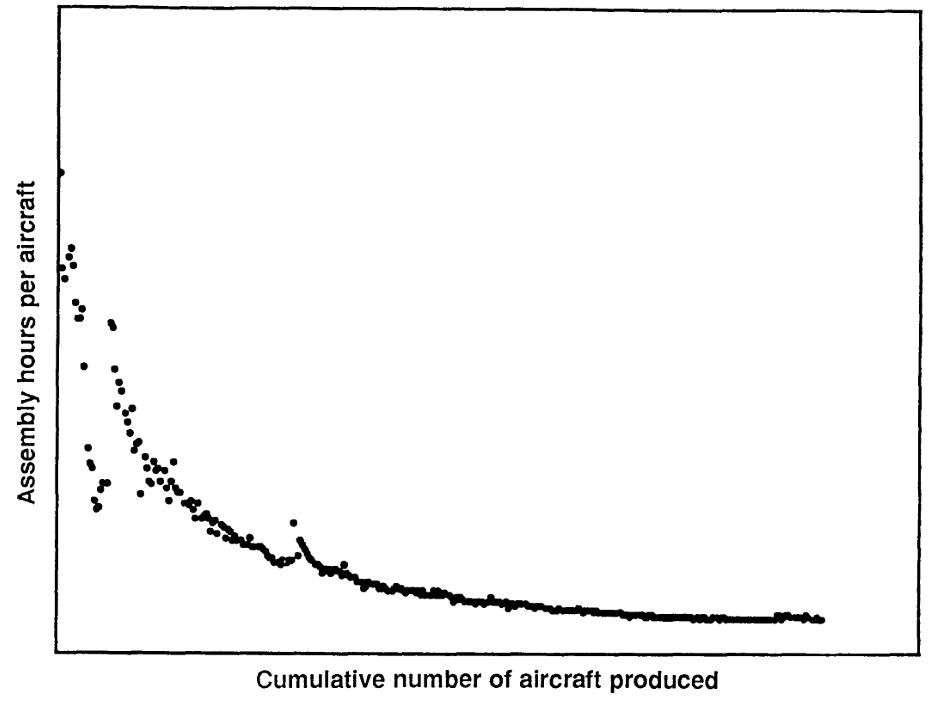
\includegraphics[height=5cm]{resources/learning_curve1.png}
		\caption{Relation between assembly hours per aircraft and cumulative number produced. Units omitted. From: \citet[p. 921]{Argote1990}}
		\note{You have probably seen this before. Read out caption. So in our context, we could imagine an organization operating its pipeline and equipment, getting better at it, making less mistakes, having less incidents. The organization in charge of pipeline safety is a suborganization.}
	\end{figure}
\end{frame}

\begin{frame}
	\frametitle{\insertsection}
	\framesubtitle{Disrupted learning}
	\begin{figure}
		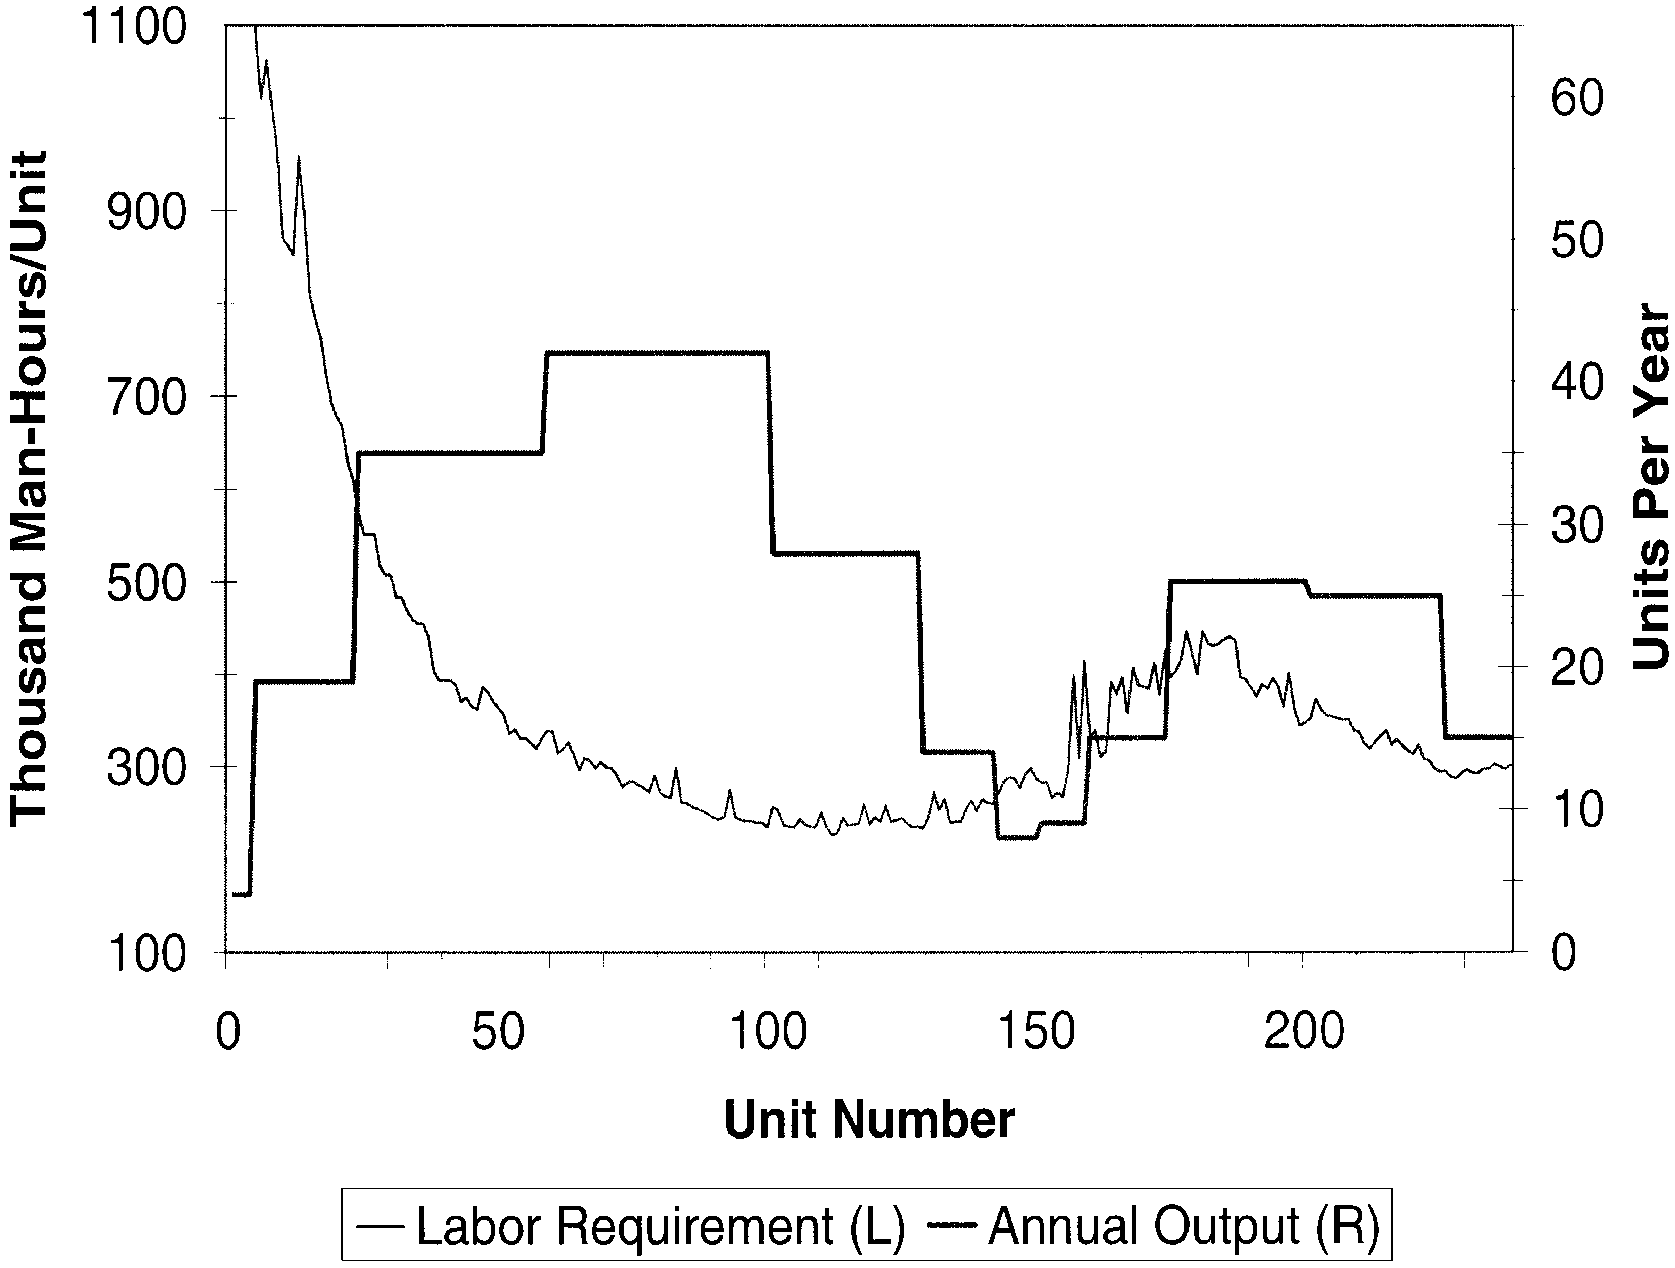
\includegraphics[height=5cm]{resources/learning_curve2.png}
		\caption{L-1011 Production: Direct Labor Requirement and Yearly Output. From: \citet[p. 1039]{Benkard2000}}
	\end{figure}
	\note{We see more than in the last picture. This is the production of the Lockheed L-1011. Famous for being an amazing plane, but a commercial failure. What happend here, around 150 units? Economic downturn, production was disrupted. Then, company decided the only way to break even is to produce a certain number of planes, but that did not happen.}
\end{frame}

\begin{frame}
	\frametitle{\insertsection}
	\framesubtitle{Disrupted learning}
	\begin{figure}
		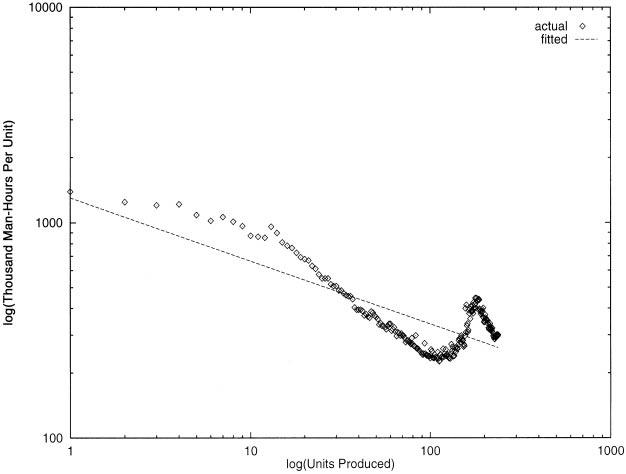
\includegraphics[height=5cm]{resources/learning_curve3.jpg}
		\caption{Traditional Learning Curve: All 238 (log-log). From: \citet[p. 1046]{Benkard2000}}
	\end{figure}
	\note{This is what actually happened. After Lockheed increased production again, the number of man-hours per plane actually increased for a while, before it decreased again. In our context, we could imagine a pipeline operator operating a pipeline for many years, then shutting it off for a while, before resuming operations. Knowledge would be lost, especially if the shut-off went hand in hand with lay-offs, and if the company had to hire new staff later.}
\end{frame}

\begin{frame}
	\begin{block}{}
		\Huge Organizational forgetting
		\bigbreak		
		\normalsize Also known as knowledge depreciation
		\note{The Lockheed is a pretty famous example for this.}
	\end{block}{}
\end{frame}

\begin{frame}
	\frametitle{Organizational forgetting}
	\begin{itemize}
		\item Turnover \citep{DeHolan2004,Rao2006}
		\note{Relate sources of forgetting to our context.\medbreak When a large number and/or key employees leave a company, and knowledge and/or networks are lost as a result. Which is also acknowledges in the wider learning literature.\medbreak}
		\item Loss of recorded knowledge
		\item Technology becoming irrelevant
		\item Decay of social networks \citep{Argote2013_3,Argote1990,Thompson2007}
		\item Disruption
		\item 
		\begin{itemize}
			\item Internal
				\begin{itemize}
					\item Disruption of regular production 
					\item Technology \citep{Amburgey1993,Edmondson2001}
					\item Restructuring/reorganization/layoffs (or even hirings) \citep{Benkard2000,Anderson2014}
				\end{itemize}
			\item External
				\begin{itemize}
					\item Economic cycles \citep{Rockart2019}
					\item Natural disasters \citep{Anderson2014}
				\end{itemize}
		\end{itemize}
	\end{itemize}
	\note{Organizational disruption is special case of organizational forgetting. Disruption can stem from inside, or outside of the organization.}
\end{frame}




\begin{frame}
	\frametitle{Research Question}
	How does organizational learning and forgetting play out in the context of strategic adjustment and hierarchies?
	\note{Let me show you the phenomenon I have been working on, what I believe is going on, and how that generalizes.}
\end{frame}

\begin{frame}
	hello world
\end{frame}

\begin{frame}[allowframebreaks]
	\frametitle{Bibliography}
	\bibliography{bibliography}
	\bibliographystyle{chicago}
\end{frame}

\end{document}